\lstinputlisting[language=bash,basicstyle=\small]{python_codes/fieldstone_92/keywords.ascii}

\begin{center}
Code at \url{https://github.com/cedrict/fieldstone/tree/master/python_codes/fieldstone_92}
\end{center}

\par\noindent\rule{\textwidth}{0.4pt}

%%%%%%%%%%%%%%%%%%%%%%%%%%%%%%%%%%%%%%%%%%%%%%%%%%%%%%%%%%%%%%%%%%%%%%%%%%%%%%%%%%%%%%%%%%%%%%%%%%%%


This stone solves the axisymmetric problem of the Stokes sphere in a cylinder, 
similarly to Stone 91. However, it relies on an unstructured grid with 
Crouzeix-Raviart elements (see Section~\ref{ss:XXX}).

The workflow is as follows: the main parameters are defined in {\sl parameters.py}.
The file {\sl generate\_nodes.py} uses these parameters to generate points on the 
boundary of the rectangular domain and on the half circle. 
A call to {\sl triangle} is then made and a very important additional parameter is passed
as argument to triangle: the maximum area of a triangle. 
{\sl triangle} returns the (constrained) Delaunay triangulation of these points, 
and this information is then read in by {\sl stone.py} which solves the 
Stokes equation in axisymmetric formulation (see Section~\ref{ss:XXX}). 
Boundary conditions are free slip everywhere except no slip on the right. 

All these actions are carried out automatically when the following script is 
used\footnote{It assumes that the triangle program has been compiled and 
is located outside of the fieldstone tree.}:
\begin{lstlisting}
python3 generate_nodes.py
cat mypoints mysegments > mesh.poly
../../../../triangle/triangle  -j -q -a0.00100 -o2 -pc mesh.poly
echo "nel="
head -1 mesh.1.ele 
head -1 mesh.1.ele > temp
echo "NV0="
head -1 mesh.1.node 
head -1 mesh.1.node >> temp
python3 stone.py
\end{lstlisting}

Two remarks: the code stems from another code which implemented time stepping, 
which explains there is now a single fake time step loop in it. 
Pressure normalisation is not done the right way: the pressure nullspace is 
not removed from the matrix, but the solution is later normalised so that 
its average over the domain is zero.

\begin{center}
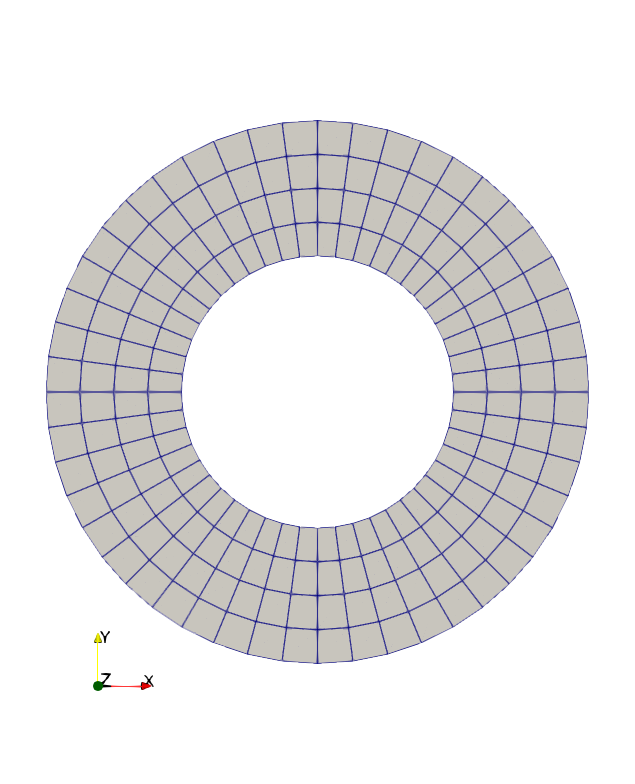
\includegraphics[width=4.3cm]{python_codes/fieldstone_92/results/mesh1}
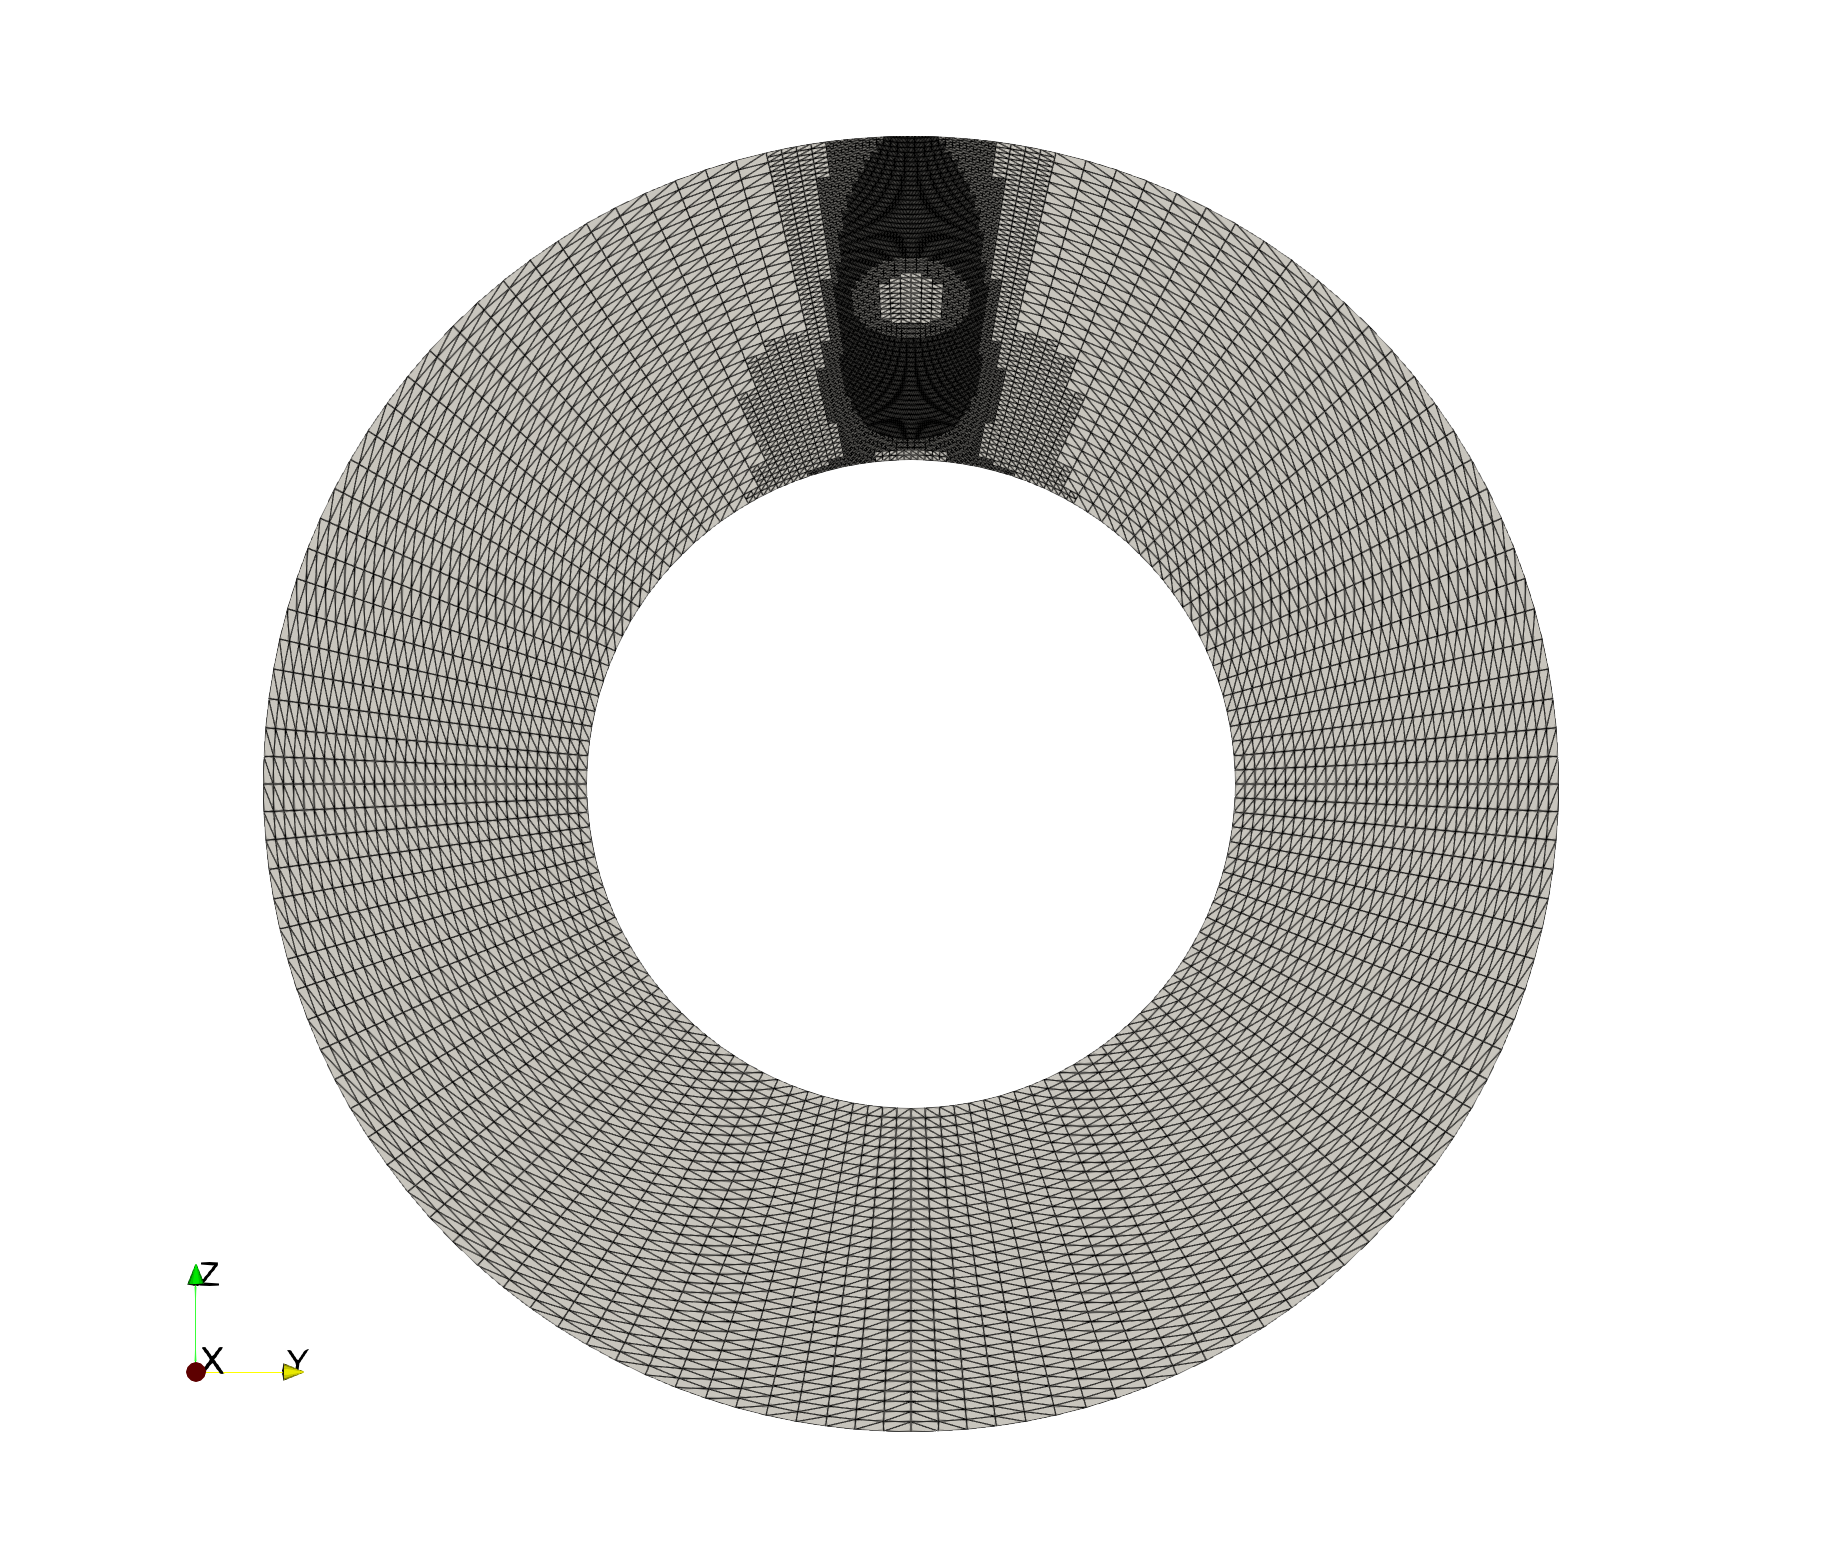
\includegraphics[width=4.3cm]{python_codes/fieldstone_92/results/mesh2}
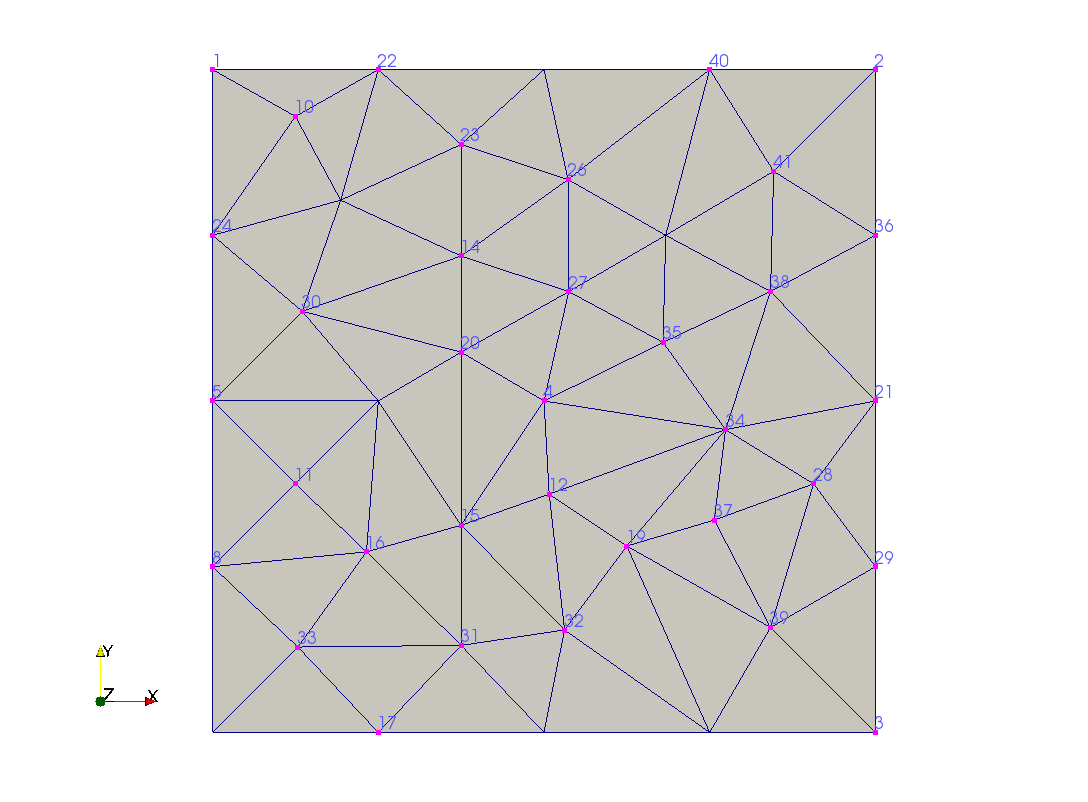
\includegraphics[width=4.3cm]{python_codes/fieldstone_92/results/mesh3}
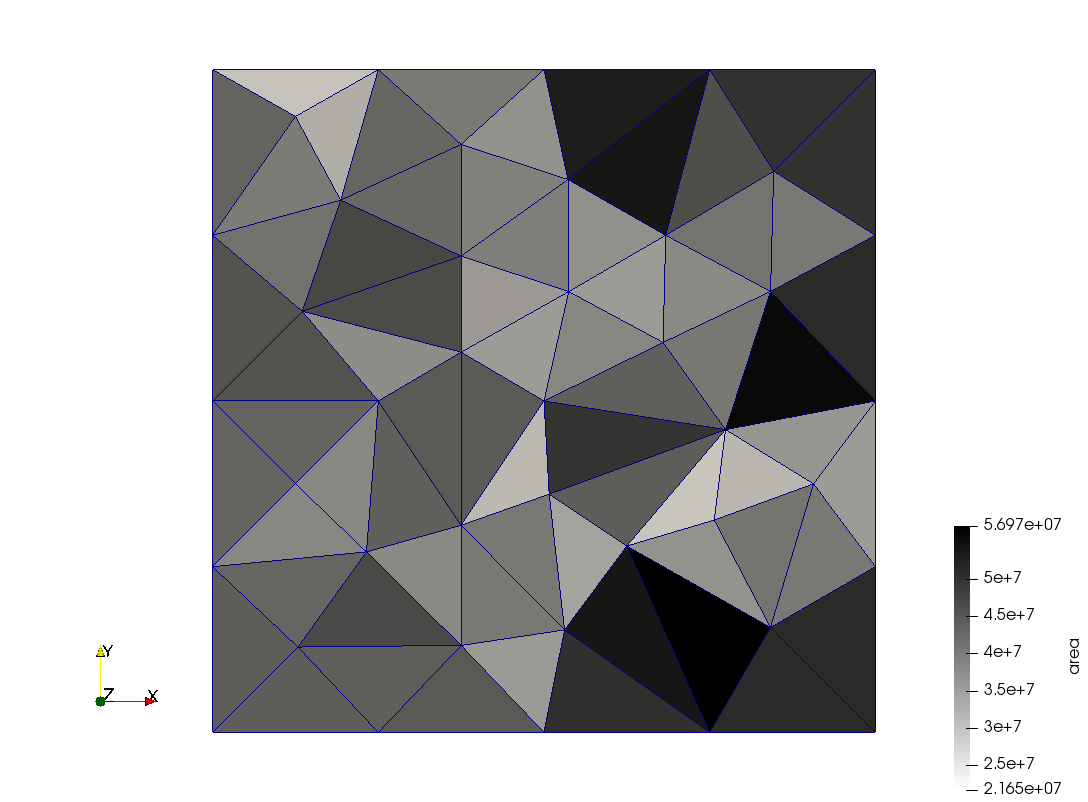
\includegraphics[width=4.3cm]{python_codes/fieldstone_92/results/mesh4}\\
{\captionfont Left to right: nel=2432,2468,2588,2866}
\end{center}


\begin{center}
\includegraphics[width=5.5cm]{python_codes/fieldstone_92/results/mat}
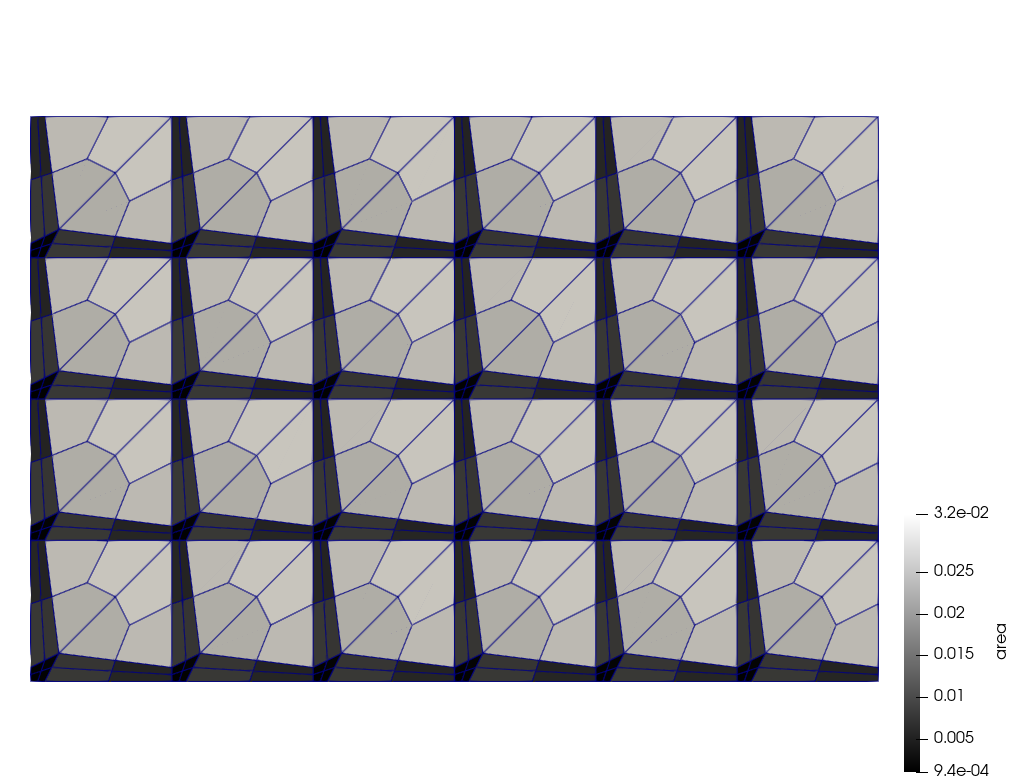
\includegraphics[width=5.5cm]{python_codes/fieldstone_92/results/area}
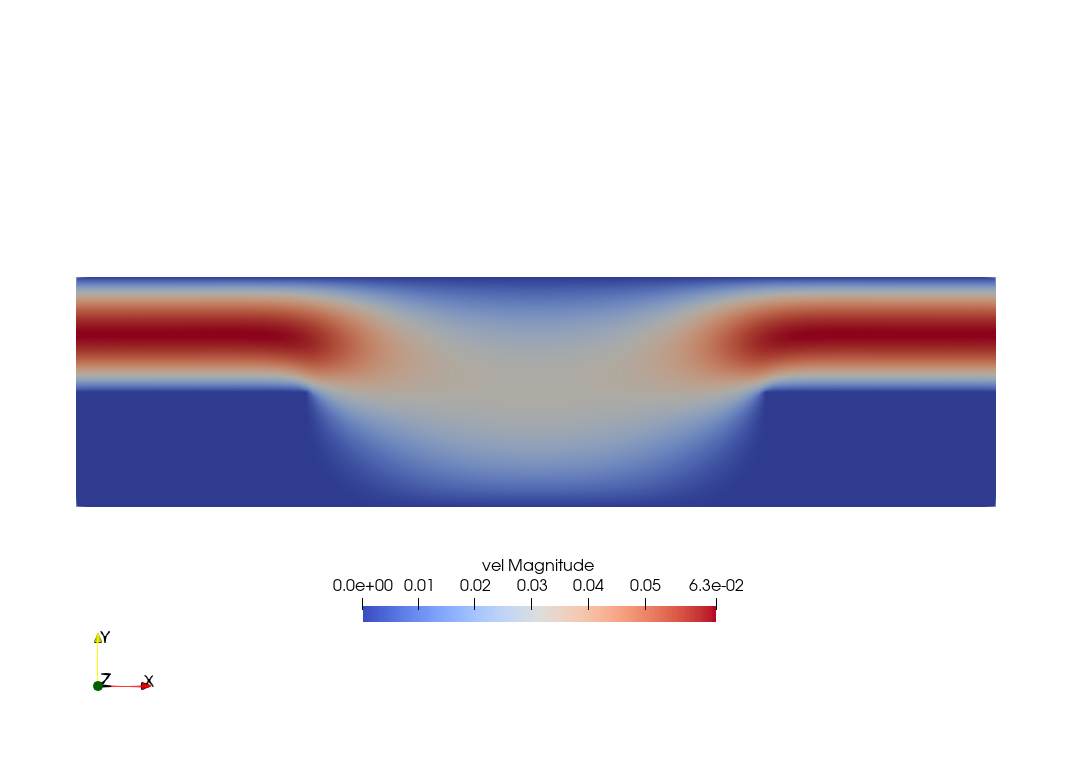
\includegraphics[width=5.5cm]{python_codes/fieldstone_92/results/vel}\\
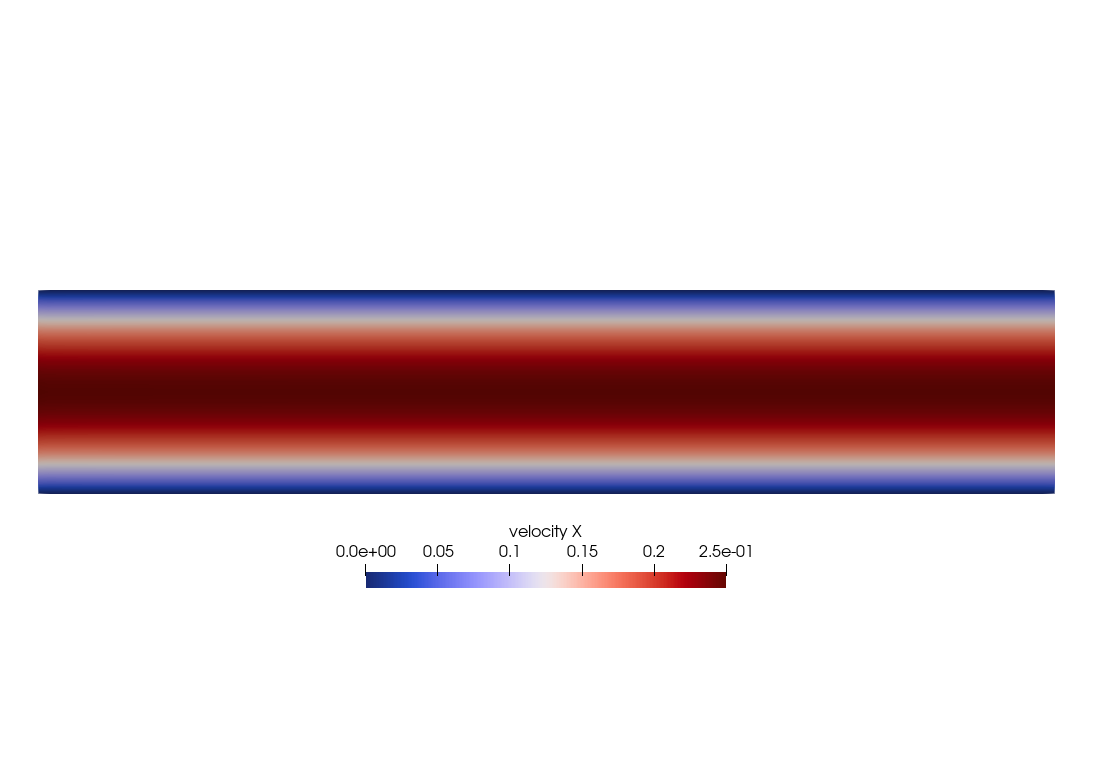
\includegraphics[width=5.5cm]{python_codes/fieldstone_92/results/u}
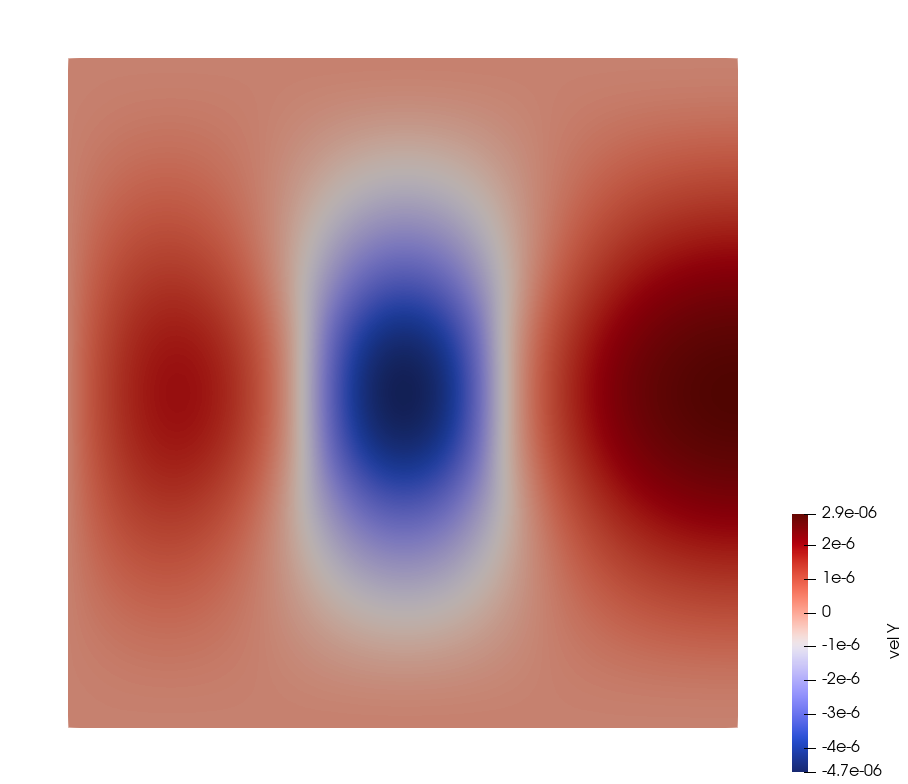
\includegraphics[width=5.5cm]{python_codes/fieldstone_92/results/v}
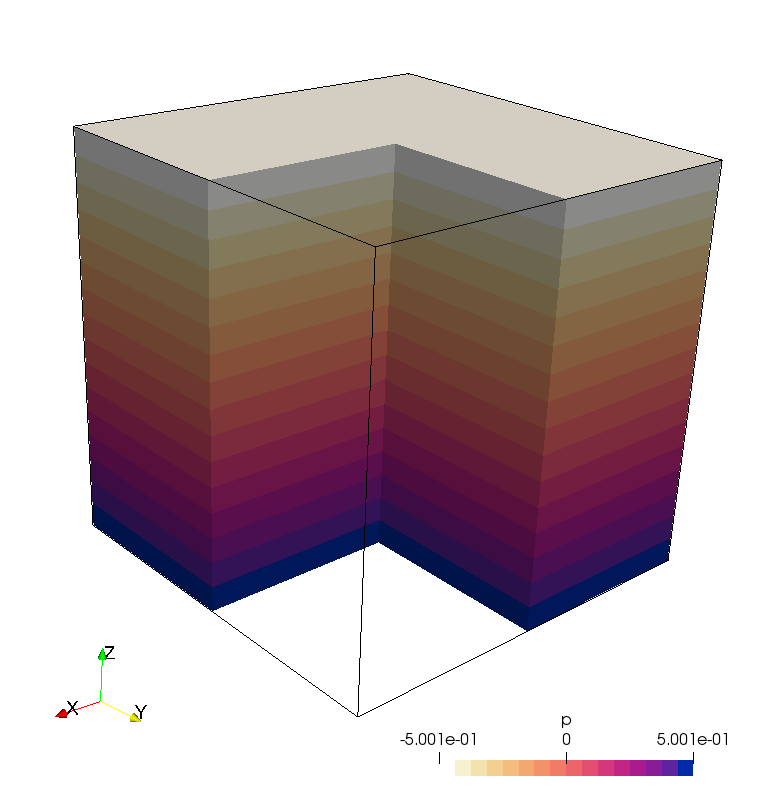
\includegraphics[width=5.5cm]{python_codes/fieldstone_92/results/press}\\
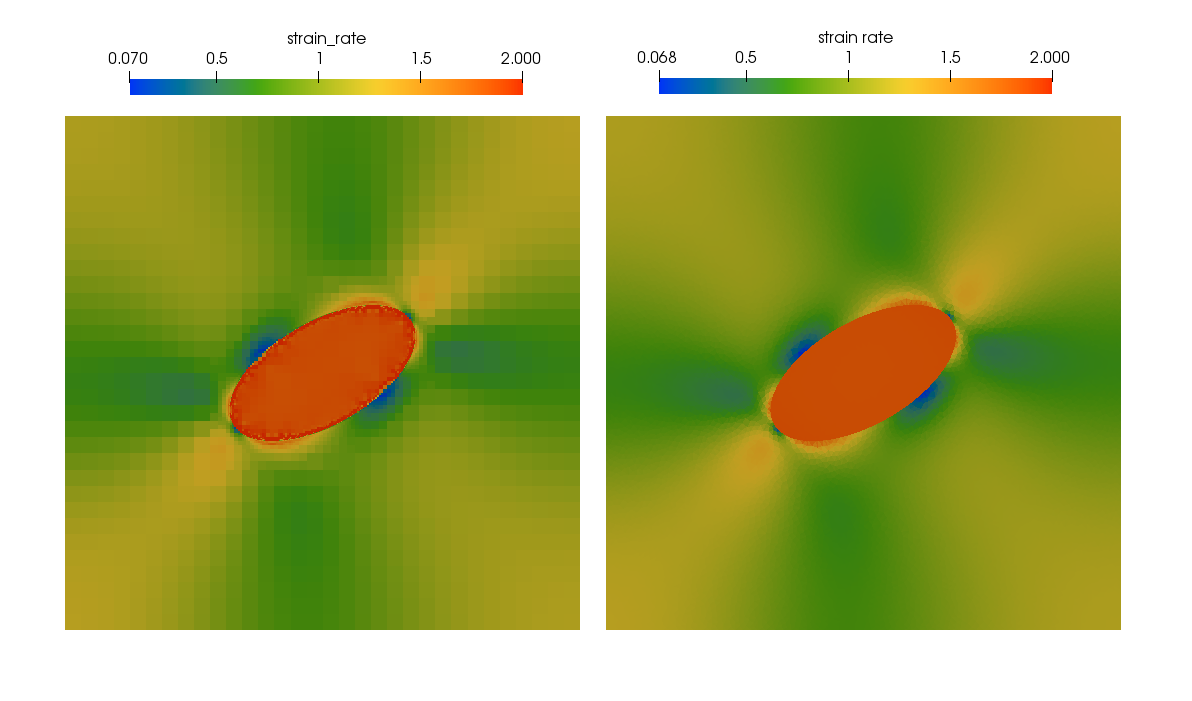
\includegraphics[width=5.5cm]{python_codes/fieldstone_92/results/sr}
\includegraphics[width=5.5cm]{python_codes/fieldstone_92/results/tauxx}
\includegraphics[width=5.5cm]{python_codes/fieldstone_92/results/tauxy}
\end{center}

Because the triangle size varies a lot within a mesh, defining a mesh size $h$
makes littel sense, so we plot the following results as a function of the 
number of elements:

\begin{center}
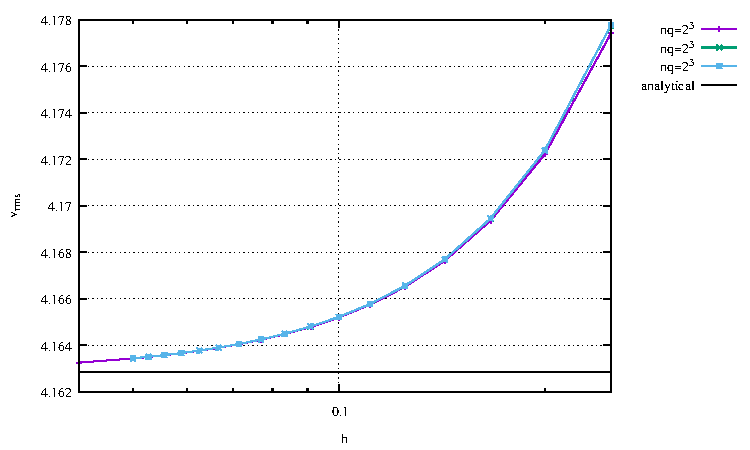
\includegraphics[width=8cm]{python_codes/fieldstone_92/results/vrms}
\includegraphics[width=8cm]{python_codes/fieldstone_92/results/vc}\\
{\captionfont Left: vrms over the whole domain for $L_y=1$; Right: 
measured velocity in the middle of the sphere. Some weird 
effect is taking place at very high resolution...}
\end{center}

The parameter $n_p$ is user defined and is an attempt to parameterise 
the resolution of the domain sides and the half circle with a single parameter.
In {\sl parameters.py} we have:
\begin{lstlisting}
np_top=n_p
np_bottom=n_p
np_left=10*n_p
np_right=5*n_p
np_sphere=10*n_p
\end{lstlisting}

We see that the sphere velocity in its middle 
matches the Habermann and Faxen values remarkably well, 
especially when the domain is made taller (top and bottom 
boundaries are further away) and the viscosity of the 
sphere is brought up to $10^5$.


\begin{center}
\includegraphics[width=8cm]{python_codes/fieldstone_92/results/stress.png}
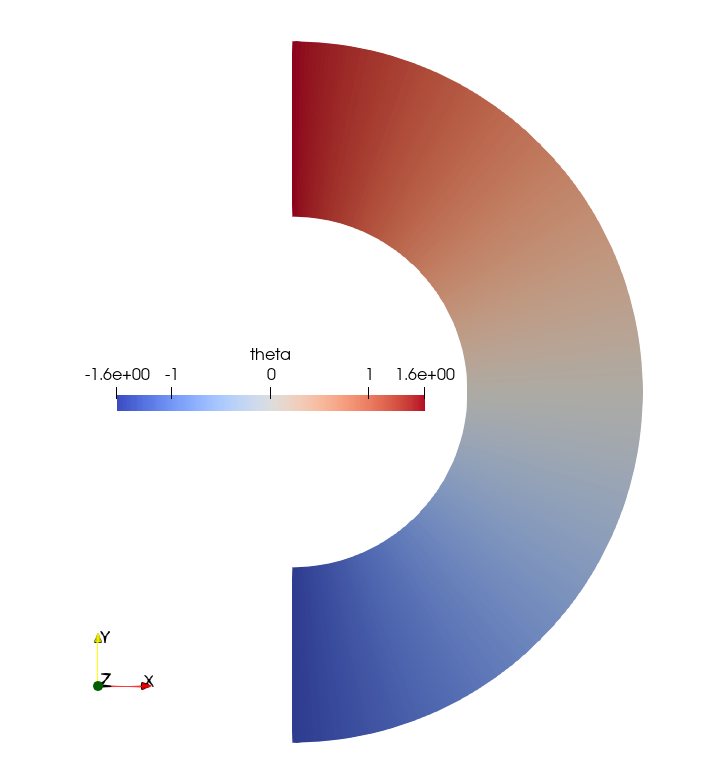
\includegraphics[width=8cm]{python_codes/fieldstone_92/results/theta.png}\\
{\captionfont Deviatoric stress principal directions (left) and angle (right).} 
\end{center}
